\chapter{Introduction}
\section{Motivation}
ATF2 is a facility build at KEK (Tsukuba, Japan) where the main objective is to confirm the local chromaticity correction scheme and to develop the required instrumentation for high energy linear accelerators.
GOALS:\par
{\Large
 \begin{itemize}
  \item Small vertical beam size ({\color{red} goal 1})
  \begin{itemize}
   \item Achieve $\sim 37$nm
   \item Validate Local chromaticity correction
  \end{itemize}
  \item Stabilization of beam center ({\color{blue} goal 2})
  \begin{itemize}
   \item down to $\sim2$nm
  \end{itemize}
 \end{itemize}
}
\subsubsection{How to achieve it?}
In order to achieve these goals at the IP (Interaction Point, which is virtual as no interaction is foreseen), the beam trajectory is measured (position, angle is obtained from two position measurements) for one first bunch and corrections on the beam trajectory are set over a second (or several) bunches.\par
It requires two BPMs to measure position and angle, and one additional to compare with. Three BPMs in total.\par
The challenge is to measure beam position to the required precision.\par
{\LARGE
  \begin{itemize}
   \item Locate BPMs to enable the \textbf{ maximum possible} beam position resolution
   \item Precision $\sim 5\mu$m
   \item Calibration to 1nm or $\sim 10^{-4}$
  \end{itemize}
 \hspace*{5cm}$\Downarrow$\\
 Displace each BPM block \textbf{independently}
 }\par
\begin{figure}[htb]
\begin{center}
  \includegraphics[angle=0,scale=0.35]{scalefactors.jpg}\caption{Scale factor required for the system.}\label{f-scalefactors}
\end{center}
\end{figure}
 \begin{figure}[htb]
\begin{center}
\includegraphics[angle=0,scale=0.2]{ATF2layout33.jpg}\caption{ATF and ATF2 layout where the final section is inside a red rectangle. Inside this rectangle is the IP.}\label{f-ATF2layout}
\end{center}
\end{figure}
\begin{figure}[htb]
\begin{center}
\includegraphics[angle=0,scale=0.16]{chambrevide.jpg}\caption{Vacuum chamber used to install 3 BPM inside. Fixed in an optical table at the IP region.}\label{f-chambrevide}
\end{center}
\end{figure}
\begin{figure}[htb]
 \begin{center}
\includegraphics[angle=0,scale=0.22]{BPMs01.jpg}\caption{3 BPMs called "IPBPMs" composing two blocks, one (PBPMA and IPBPMB) upstream and one (IPBPMC) downstream the IP.}\label{f-BPMs01}
\end{center}
\end{figure}
\begin{figure}[htb]
 \begin{center}
\includegraphics[angle=0,scale=0.0355]{IMAG0460.jpg}\caption{Photo of the mechanical assembly.}\label{f-assembly}
\end{center}
\end{figure}
  \begin{figure}[htb]
 \begin{center}
\includegraphics[angle=0,height=7.5cm,width=12cm]{interface.jpg}\caption{Description of movers direction of movement, voltage ranges and qualitative location. Each blocks moves laterally vertically indepently.}\label{f-movers}
\end{center}
\end{figure}

\section{Alignment Requirements}
Consider Figure \ref{beamdist}, where vertical position histogram is to be filled with each passing bunch. The scale is divided in $N$ parts, each one with same width. It also has a minimum and maximum values. As the beam passes, the cavity signal is going to be ideally proportional to beam centroid position $y_k$, where $k$ stands for the $k$-th bunch, all charge is concentrated there and the distribution effect is a multiplying factor. In red, it is possible to see that beam distribution might change slightly, but in general is going to be gaussian and to have same size (beam size = 1$\sigma_y$).
\begin{figure}[htb]
\begin{center}
 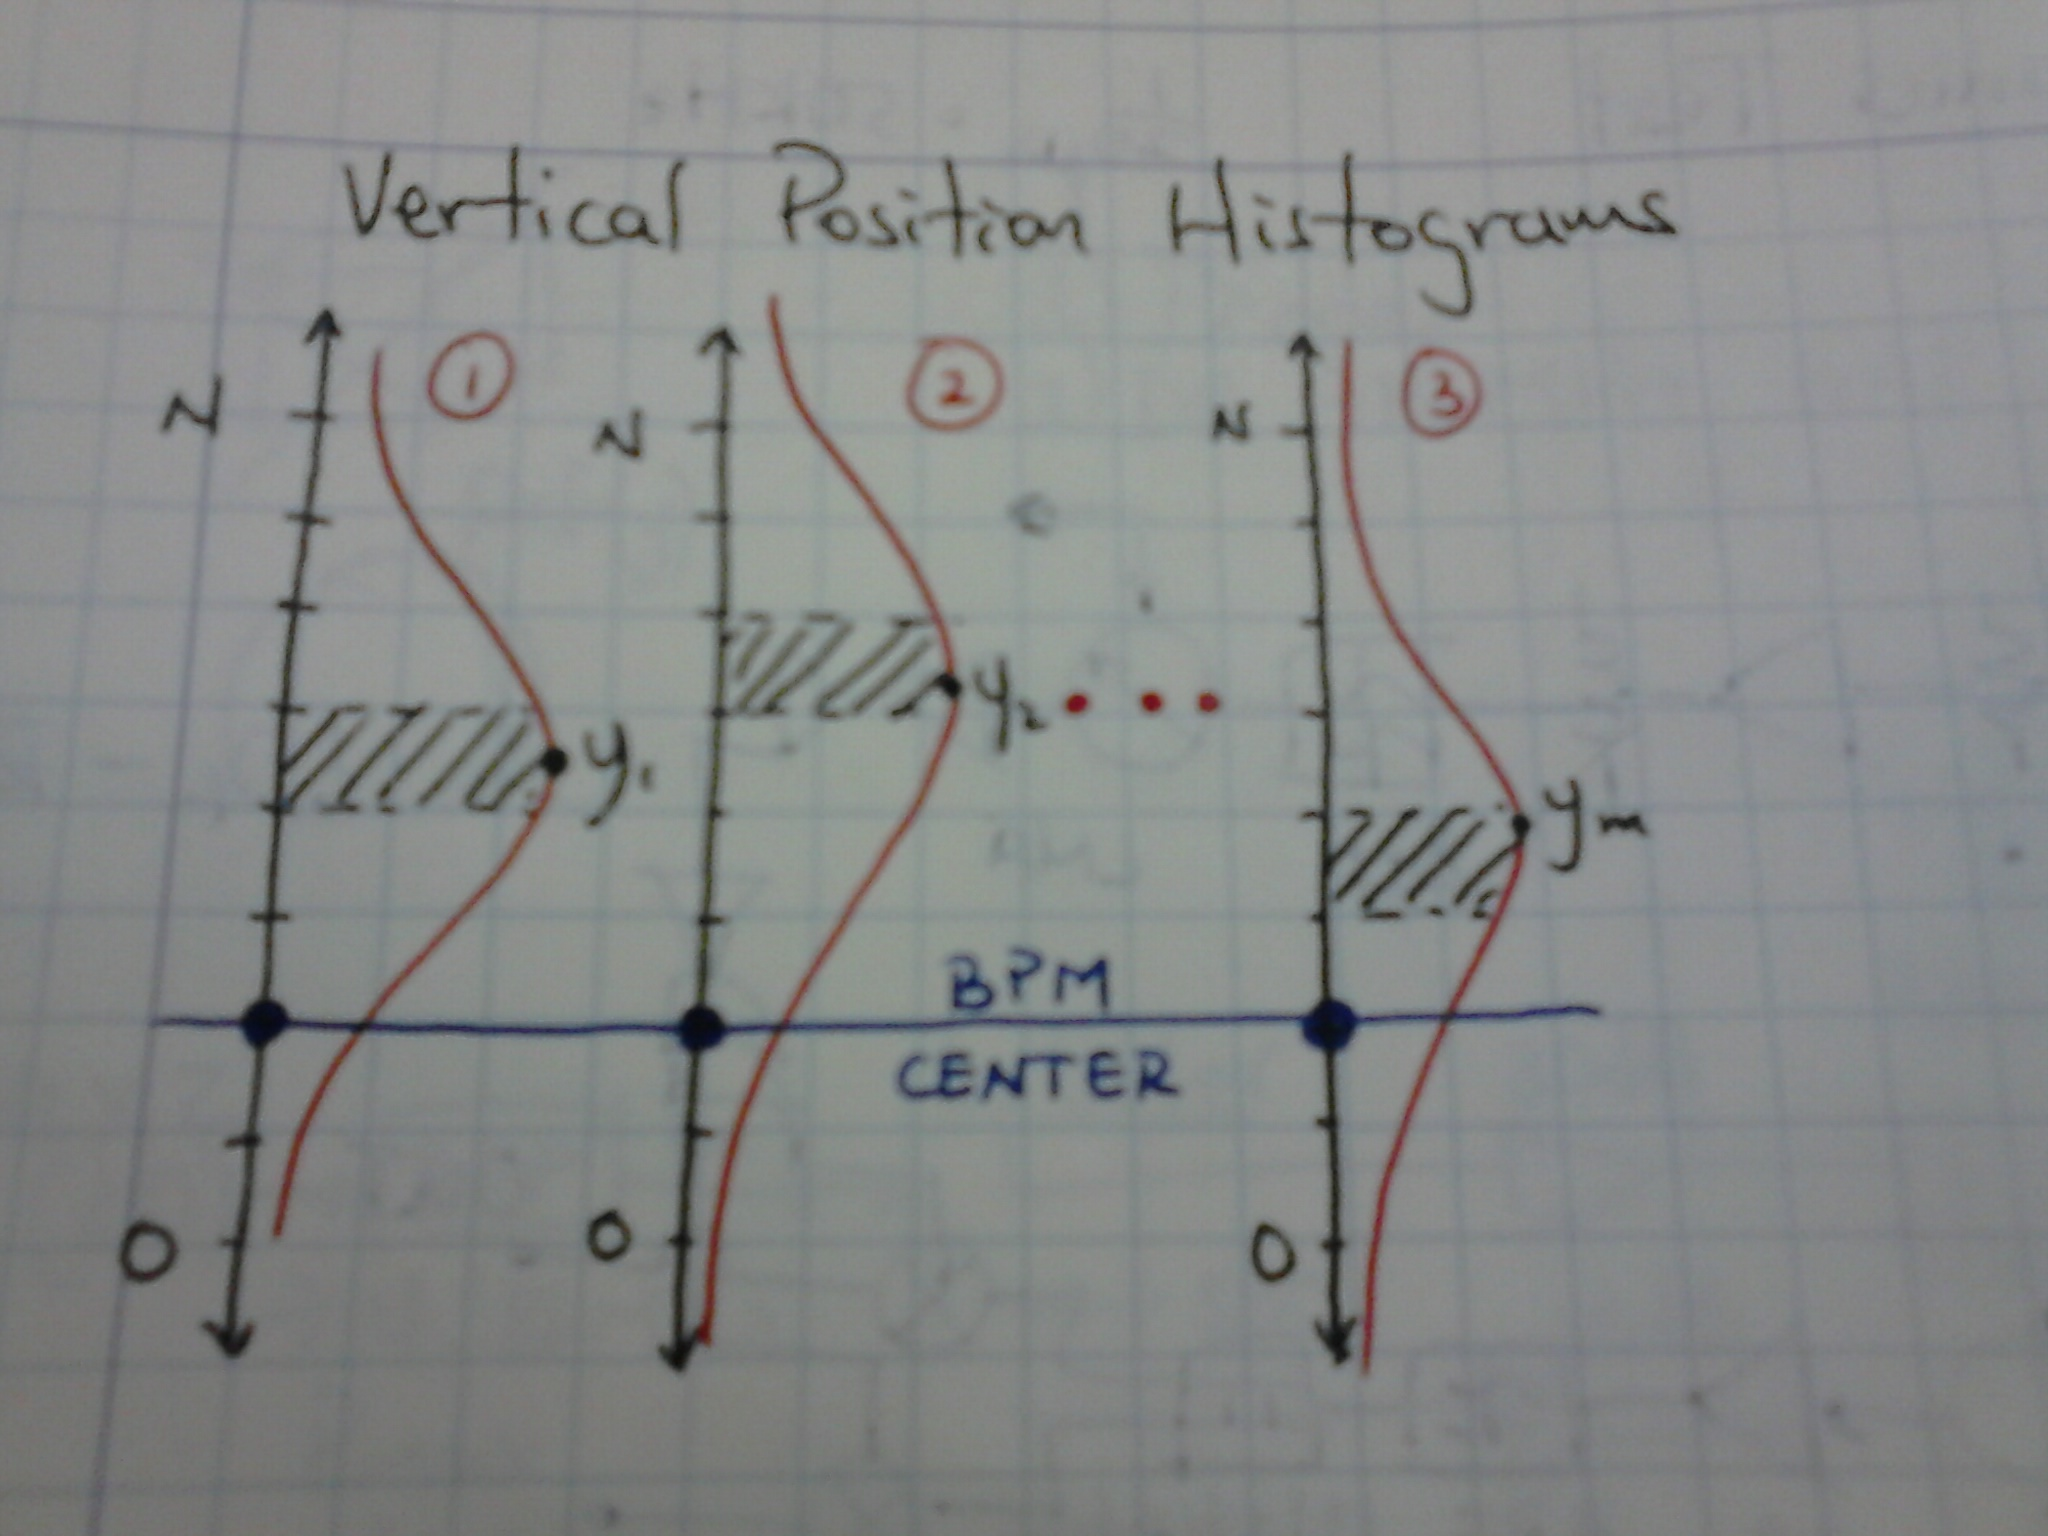
\includegraphics[angle=0,scale=0.1]{DSC_0026.jpg}\caption{Beam distr.}\label{beamdist}
 \end{center}
\end{figure}
Each vertical measurement $y_k$ is displaced from BPM center in an amount determined by a vertical offset $y_0$ with respect to cavity center and a random number proportional to beamsize ($y_{jk}=p\sigma_y$, and $p$ between 10 to 20\%, jitter). Therefore, from a sample $Y$ of $m$ bunches measured, $y_0=\langle Y\rangle$ and $\sigma_j^2=\langle Y^2\rangle-\langle Y\rangle^2$. In the case of one bunch, $y_{jk}=y_k-y_0$. Jitter will also be present in horizontal position and angles. For the moment, only discretisation level will be the only error source contributing to each $y_k$.\par
The objective is to measure $\boldsymbol{y_j}$ with \textbf{1nm} or $\boldsymbol{10^{-4}}$ relative precision for a bunch ($k$=1).\par
The preceeding statament means that the scale division used to measure $y$ should comply with\par
\begin{equation}
  \frac{y_j}{N}\leq1\text{nm, or, }\frac{1}{N}\leq10^{-4}
\end{equation}
In order to satisfy both, $N>10^{4}$. It also sets two ranges for the jitter measurement:
\begin{itemize}
 \item $y_j<10\mu$m, where resolution is below 1nm.
 \item $y_j\geq10\mu$m, where resolution is $10^{-4}$ maximum.
\end{itemize}
The maximum number counts used to measure jitter will always be below 10000. If we consider jitter conviniently centered, then it will be 5000 counts below $N/2$ and 5000 counts above $N/2$. The allowed offset under this circumstances, will be from 5000 counts to $N-5000$ counts. In total we have substracted 10000 counts from the total range, and the maximum offset will be $N-10000$ counts.\par
The number of counts $N$ comes from the binary $2^b$ discretisation scale where $b$ is the number of bits. As oscilloscopes are only 8 bits, the max. resolution will be around $10^{-2}$ ($2^8$). For a system with 14 bits, $N=16384$,  6384 counts are free for tolerances to different effects including offset. Any offset below $6.384\mu$m will will allow 1nm precision. Above this size, only $10^{-4}$ might be reached.\par
Table \ref{toletab} shows the different level of tolerances corresponding to different precision levels for 1nm resolution and 14 bits discretisation.\par
\begin{table}[hbt]
\begin{center}
 \begin{tabular}{|c|c|c|}\hline
 Precision & Total OFFSET SIGNAL ($\mu$m) & Centered ($\mu$m)\\\hline
 $10^{-2}$ &16.824&$\pm$8.142 \\\hline
 $10^{-3}$ &15.384&$\pm$7.692\\\hline
 $10^{-4}$ &6.384&$\pm$3.192\\\hline
 \end{tabular}
 \caption{Tolerances and precision.}\label{toletab}
 \end{center}
\end{table}
Consider now the signal $S$ as the sum of the two outputs from the cavity (which are ideally 180\degre separated) as seen in figure \ref{Ssignal},\par
\begin{figure}[htb]
 \begin{center}
  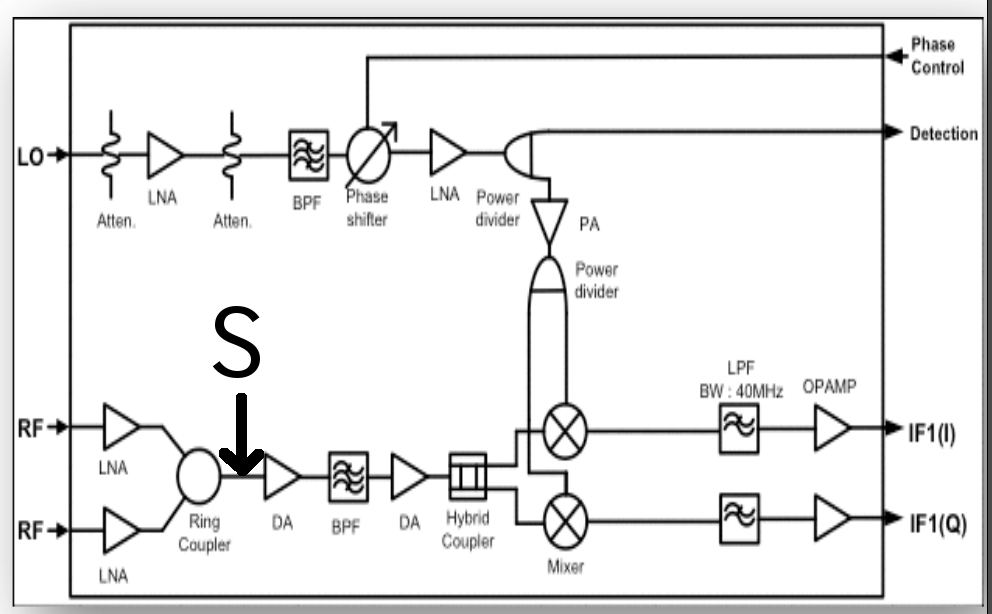
\includegraphics[angle=0,scale=0.4]{electr2.jpg}\caption{Signal S.}\label{Ssignal}
 \end{center}
\end{figure}
Signal $S$ for the vertical outputs of one BPM and one bunch is composed of:
\begin{equation}
S = y+is_p\theta_p+s_{xy}(x+is_y\theta_y)+x\theta_r
\end{equation}
where $i$ is the imaginary number indicating a 90 degrees phase difference (angle signals have 90 phase difference with respect to position signals from cavity). $s_p$ is the sensitivity to pitch angle, $s_{xy}$ is the inverse of X-Y isolation, $s_y$ is the yaw angle sensitivity. $x,y,\theta_p,\theta_r,\theta_y$, are horizontal position, vertical position, pitch, roll and yaw angles BPM with respect to beam.\par
Signal $S$ can be separated in real and imaginary parts:
\begin{equation}
S = (y+s_{xy}x+x\theta_r)+i(s_p\theta_p+s_{xy}s_y\theta_y)
\end{equation}
This signals are rotatated by an arbitrary angle $\phi$ to obtain the $I'$ and $Q'$ at the phase shifter block.
\begin{align*}
S &= \underbrace{(y+s_{xy}x+x\theta_r)(\cos\phi+i\sin\phi)}+\underbrace{i(s_p\theta_p+s_{xy}s_y\theta_y)(\cos\phi+i\sin\phi)}\\
  &= I' + Q' 
\end{align*}
In the case of perfect IQ rotation ($\phi=0$), all imaginary (angle and others) component is removed from real (position) component in the $S$ signal. However, in practice this rotation could be achieved to precision set by $\Delta\phi$, then, to first order
\begin{equation}
S=[(y+s_{xy}x+x\theta_r)-\Delta\phi(s_p\theta_p+s_{xy}s_y\theta_y)]+i[\Delta\phi(y+s_{xy}x+x\theta_r)+(s_p\theta_p+s_{xy}s_y\theta_y)]
\end{equation}
At this point will be only interested in the real part as it contains most of the vertical position signal.
\begin{equation}
 \Re[S]=S_y = (y+s_{xy}x+x\theta_r)-\Delta\phi(s_p\theta_p+s_{xy}s_y\theta_y)
\end{equation}
The last equation shows the contribution to vertical signal from the relative position BPM to beam.\par
Mean value of $S_y$ signal over $m$ bunches sample will be equal to
\begin{equation}
 \langle S_y\rangle = [y_0+(x_0+\eta\delta)(s_{xy}+\theta_{r0})]-\Delta\phi[s_p\theta_{p0}+s_{xy}s_y(\theta_{y0}+\eta'\delta)]
\end{equation}
where all 0-index correspond to misaligment, $\eta$ and $\eta'$ are the dispersion and dispersion angle optic parameters, $\delta=10^{-3}$ is the energy spread, and no beam rotation is considered. $\langle S_y\rangle$ contribution to signal should be then below the values listed in Table \ref{toletab}.\par
The signal jitter $\sigma_{S_y}^2=\langle S_y^2\rangle-\langle S_y\rangle^2$ will come from
\begin{align*}
 \sigma_{S_y}^2=&\sigma_{jy}^2+\sigma_{jx}^2[s_{xy}+\theta_{r0}]^2+(\Delta\phi)^2[s_p^2\sigma_{jy'}^2+s_{xy}^2s_y^2\sigma_{jx'}^2]\\
 =&\langle y^2\rangle-y_0^2+(\langle x^2\rangle-x_0^2)[s_{xy}+\theta_{r0}]^2+(\Delta\phi)^2[s_p^2(\langle y'^2\rangle-y'^2_0 +s_{xy}^2s_y^2(\langle x'^2\rangle-x'^2_0)]
\end{align*}
and substracting all means effects
\begin{equation}
 \sigma_{S_y}^2=\langle y^2\rangle+\langle x^2\rangle[s_{xy}+\theta_{r0}]^2+(\Delta\phi)^2[s_p^2\langle y'^2\rangle+s_{xy}^2s_y^2(\langle x'^2\rangle)]
\end{equation}
In the case of one single bunch and known substracted means, the signal jitter will be
\begin{equation}
 %S_j=y_j-y_0+(x_j-x_0)(s_{xy}+\theta_{r0})+\Delta\phi[s_p(y'_j-y'_0)+s_{xy}s_y(x'_j-x_0)]
 S_j=y_j+x_j(s_{xy}+\theta_{r0})+|\Delta\phi|(s_py'_j+s_{xy}s_yx'_j)
\end{equation}
from where it is possible to conclude that roll angle $\theta_{r0}$ and phase shifter precision $\Delta\phi$ limit directly the jitter measurement.\par
Isolation X-Y (1/$s_{xy}$) was measured to be under 50dB (Pin/Pout$<10^{-5}=3.162\times10^{-3}$ voltage isolation), sensitivity to pitch ($s_p$) was measured to be $3.2\mu$m/mrad, and sensitivity to yaw ($s_y$) is 2.9$\mu$m/mrad estimated in similar way to $s_p$. Precision on phase rotation ($\Delta\phi$) is still to be determined. Expresing the previous equation in nm and $\mu$rad (unless noted), we obtain
\begin{equation}
 S_j=y_j+x_j(1.880\times10^{-3}+10^{-6}\theta_{r0})+10^{-6}|\Delta\phi|(3.2y'_j+5.453\times10^{-3}x'_j)
\end{equation}
where  the BPM vertical (3.7mV/$\mu$m/nC) and horizontal (2.2mV/$\mu$m/nC) sensitivities have been used to translate voltage isolation X-Y to position scale.
% In order to have 1nm contribution from each one of these parameters, then, values should comply with
% \begin{equation}
%  x_j(\text{nm})\leq 531,\qquad \theta_{r0}(\text{mrad})\leq\frac{10^3}{x_j}, \qquad |\Delta\phi|(\text\degre)\leq\frac{57.30}{3.2y'_j+5.453\times10^{-3}x'_j}
% \end{equation}

\subsection{Mechanical resolution}
From this point, it will be assumed that mechanical positions could be measured within an absolute error shown in Table \ref{mechprec}.\par
\begin{table}[htb]
\begin{center}
 \begin{tabular}{|c|c|}\hline
  Axis (Symbol) & Mechanical Precision ($\mu$m)\\\hline
  Vertical ($\Delta y$)& 1\\
  Horizontal ($\Delta x$) & 5\\
  Longitudinal ($\Delta z$) & 5 \\\hline
 \end{tabular}\caption{Position mechanical precision}\label{mechprec}
 \end{center}
\end{table}
Assuming that angles can be estimated from two coplanar points in the BPM, then, minimum resolvable angle might be within the values shown in Table \ref{angleprec}. Figure \ref{PAcontrol} shows the approximate location of angle control points.\par
\begin{table}[htb]
 \begin{center}
  \begin{tabular}{|c|c|c|}\hline
  Angle (Symbol) & Estimated min. resolvable value (mrad) & Distance between points (mm)\\\hline
   Pitch ($\Delta\theta_p$)&0.042&120\\
   Yaw ($\Delta\theta_y$)&0.042&120\\
   Roll ($\Delta\theta_r$)&0.033&30\\\hline
  \end{tabular}\caption{Angle mechanical precision}\label{angleprec}
 \end{center}
\end{table}
\begin{figure}[htb]
 \begin{center}
  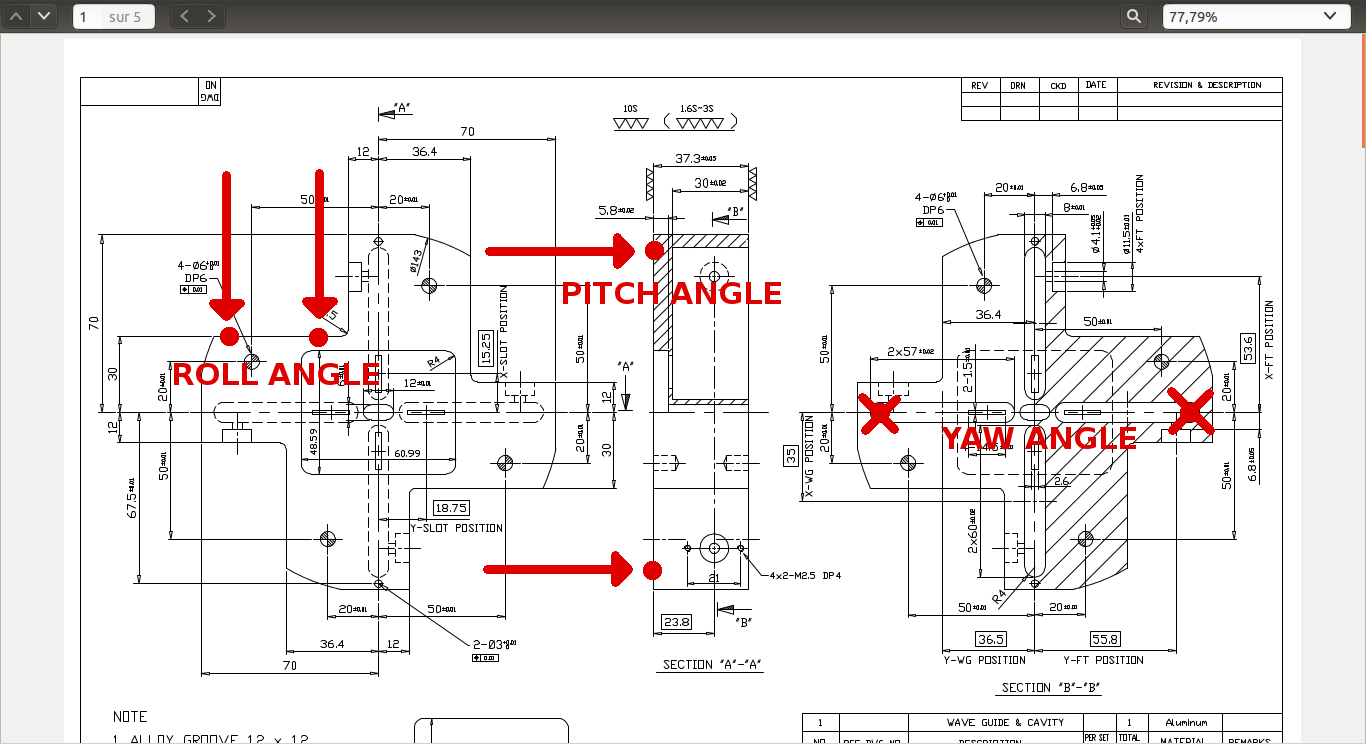
\includegraphics[angle=0,scale=0.4]{angles.jpg}\caption{Points of position and angle control.}\label{PAcontrol}
 \end{center}
\end{figure}


\subsection{Measurement cases}
\subsubsection{Beam waist at BPM using 1BX1BY and 10BX1BY optics}
Using the nominal optics 1BX1BY, the jitter will be acording to table \ref{t-jitter1BX1BY}
\begin{table}[hbt]
\begin{center}
 \begin{tabular}{|c|c|c|}\hline
 Jitter &10\% & 20\%\\\hline
 $\sigma_{yj}$(nm) & 3  & 7\\\hline
 $\sigma_{xj}$(nm) &283&565 \\\hline
 $\sigma_{y'j}$($\mu$rad) &34&69\\\hline
 $\sigma_{x'j}$($\mu$rad) &71&141\\\hline
 \end{tabular}
 \caption{Jitter with 1BX1BY optics at IP}\label{t-jitter1BX1BY}
 \end{center}
\end{table}
\begin{table}[hbt]
\begin{center}
 \begin{tabular}{|c|c|c|}\hline
 Jitter &10\% & 20\%\\\hline
 $\sigma_{yj}$(nm) & 3  & 7\\\hline
 $\sigma_{xj}$(nm) &894&1787 \\\hline
 $\sigma_{y'j}$($\mu$rad) &34&69\\\hline
 $\sigma_{x'j}$($\mu$rad) &22&44\\\hline
 \end{tabular}
 \caption{Jitter with 10BX1BY optics at IP}\label{t-jitter10BX1BY}
 \end{center}
\end{table}
therefore, The signal jitter will be
\begin{align*}
 S_j&=y_j+x_j(s_{xy}+\theta_{r0})+|\Delta\phi|(s_py'_j+s_{xy}s_yx'_j)\\
 &=7+565(1.880\times10^{-3}+10^{-6}\theta_{r0})+10^{-6}|\Delta\phi|(3.2\times69+5.453\times10^{-3}\times141)\\
 &=8+565\times10^{-6}\theta_{r0}+221\times10^{-6}|\Delta\phi|
\end{align*}
Then $\theta_{r0}\leq 1.770$mrad and $|\Delta\phi|\leq 4.525$mrad=0.256\degre are required to 1nm resolution.\par
Using the nominal optics 10BX1BY, the jitter will be acording to table \ref{t-jitter10BX1BY}
\begin{align*}
 S_j&=7+1787(1.880\times10^{-3}+10^{-6}\theta_{r0})+10^{-6}|\Delta\phi|(3.2\times69+5.453\times10^{-3}\times22)\\
 &=10+1787\times10^{-6}\theta_{r0}+221\times10^{-6}|\Delta\phi|
\end{align*}
Then $\theta_{r0}\leq 0.556$mrad and $|\Delta\phi|\leq 4.525$mrad=0.256\degre are required to 1nm resolution.\par
The two more restrictive values will be taken to calculate the tolerances to misaligment ($\theta_{r0}= 0.556$mrad and $|\Delta\phi|= 4.525$mrad=0.256\degre).
Using again the signal mean with the horizontal dispersion and horizontal dispersion angle,  $\eta=0\mu$m, $\eta'=139.6$mrad, for energy spread $\delta=10^{-3}$, then, in $\mu$m and mrad
\begin{align*}
  \langle S_y\rangle =& [y_0+(x_0+\eta\delta)(s_{xy}+10^{-3}\theta_{r0})]-10^{-3}\Delta\phi[s_p\theta_{p0}+s_{xy}s_y(\theta_{y0}+\eta'\delta)]\\
 =& y_0+2.436\times10^{-3}x_0-14.5\times10^{-3}\theta_{p0}+24.67\times10^{-6}\theta_{y0}+3.444\times10^{-6}\\
 =&1.013\Delta y
\end{align*}
where the mean is the maximum dynamic range permissible, $\Delta y$ is the vertical measurement tolerances, longitudinal and horizontal tolerances are supposed to be 5 times bigger, and angles have been replaced by the tolerances one the two points measurements and its distances. As a result, the tolerance in vertical position should be slightly below dynamic range used.\par
From columns <ADC resolution, nm/ADC> and <maximum/Dynamic Range> for beam intensity $10^{10}$ in Figure \ref{f-dynrange-KNU}, it is possible to say that measurement of control points vertical resolution with high than 10$\mu$m is acceptable and above $3\mu$m resolution is ideal. Horizontal and longitudinal resolutions will be higher than 50$\mu$m acceptable and $9\mu$m ideal.
\subsubsection{Beam waist at IP and readings in IPBPMA using 1BX1BY and 10BX1BY optics}
Using the nominal optics 1BX1BY, the jitter will be acording to table \ref{t-jitter1BX1BY-IPA}
\begin{table}[hbt]
\begin{center}
 \begin{tabular}{|c|c|c|}\hline
 Jitter &10\% & 20\%\\\hline
 $\sigma_{yj}$(nm) & 5766  &11531\\\hline
 $\sigma_{xj}$(nm) &11866&23733 \\\hline
 $\sigma_{y'j}$($\mu$rad) &0&0\\\hline
 $\sigma_{x'j}$($\mu$rad) &1&3\\\hline
 \end{tabular}
 \caption{Jitter with 1BX1BY optics at IPA}\label{t-jitter1BX1BY-IPA}
 \end{center}
\end{table}
\begin{table}[hbt]
\begin{center}
 \begin{tabular}{|c|c|c|}\hline
 Jitter &10\% & 20\%\\\hline
 $\sigma_{yj}$(nm) &5766&11531\\\hline
 $\sigma_{xj}$(nm) &3856&7713\\\hline
 $\sigma_{y'j}$($\mu$rad) &0&0\\\hline
 $\sigma_{x'j}$($\mu$rad) &5&10\\\hline
 \end{tabular}
 \caption{Jitter with 10BX1BY optics at IPA}\label{t-jitter10BX1BY-IPA}
 \end{center}
\end{table}
therefore, The signal jitter will be
\begin{align*}
S_j&=y_j+x_j(s_{xy}+\theta_{r0})+|\Delta\phi|(s_py'_j+s_{xy}s_yx'_j)\\
 &=11531+23733(1.880\times10^{-3}+10^{-6}\theta_{r0})+10^{-6}|\Delta\phi|5.453\times10^{-3}\times3\\
 &=11576+23.7\times10^{-3}\theta_{r0}+16\times10^{-9}|\Delta\phi|
\end{align*}
Then $\theta_{r0}\leq 42\mu$rad and $|\Delta\phi|\leq 63$rad are required to 1nm resolution. Tolerance in phase shifter indicates negligible beam angle effect. However, in order to check the roll angle, position must be check below 1$\mu$m precision. This is just  under mechanical checkings. Here, either we loose vertical jitter precision by a factor 10 in order to reach the vertical precision limit of 1$\mu$m or movers are required.\par
Using the nominal optics 10BX1BY, the jitter will be acording to table \ref{t-jitter10BX1BY-IPA}
\begin{align*}
S_j&=y_j+x_j(s_{xy}+\theta_{r0})+|\Delta\phi|(s_py'_j+s_{xy}s_yx'_j)\\
 &=11531+7713(1.880\times10^{-3}+10^{-6}\theta_{r0})+10^{-6}|\Delta\phi|5.453\times10^{-3}\times10\\
 &=11545+7.713\times10^{-3}\theta_{r0}+54\times10^{-6}|\Delta\phi|
\end{align*}
Again, tolerance in phase shifter $\Delta\phi$ is large as angle signal is negligible. $\theta_{r0}\leq 0.130$mrad is required to 1nm resolution.\par
The result from 1BX1BY optics will not be used as it is beyond mechanical checkings. The case 10BX1BY will be taken to calculate the tolerances to misaligment ($\theta_{r0}= 0.130$mrad). For $\Delta\phi$, a value of 100mrad will be assumed.\par
Using again the signal mean with the horizontal dispersion and horizontal dispersion angle,  $\eta=20.99\times10^{3}\mu$m, $\eta'=139.6$mrad, for energy spread $\delta=10^{-3}$, then, in $\mu$m and mrad
\begin{align*}
  \langle S_y\rangle =& [y_0+(x_0+\eta\delta)(s_{xy}+10^{-3}\theta_{r0})]-10^{-3}\Delta\phi[s_p\theta_{p0}+s_{xy}s_y(\theta_{y0}+\eta'\delta)]\\
 =& y_0+2.010\times10^{-3}x_0+42\times10^{-3}-0.320\theta_{p0}+545\times10^{-6}\theta_{y0}+0.071\times10^{-6}\\
 =&1.023\Delta y
\end{align*}
where the mean is the maximum dynamic range permissible, $\Delta y$ is the vertical measurement tolerances, longitudinal and horizontal tolerances are supposed to be 5 times bigger, and angles have been replaced by the tolerances one the two points measurements and its distances. As a result, the tolerance in vertical position should be slightly below dynamic range used.\par
From columns <ADC resolution, nm/ADC> and <maximum/Dynamic Range> for beam intensity $10^{10}$ in Figure \ref{f-dynrange-KNU}, it is possible to say that measurement of control points with vertical resolution higher than 10$\mu$m is acceptable and above $3\mu$m resolution is ideal. Horizontal and longitudinal resolutions will be higher than 50$\mu$m acceptable and $9\mu$m ideal.
\begin{figure}[htb]
 \begin{center}
  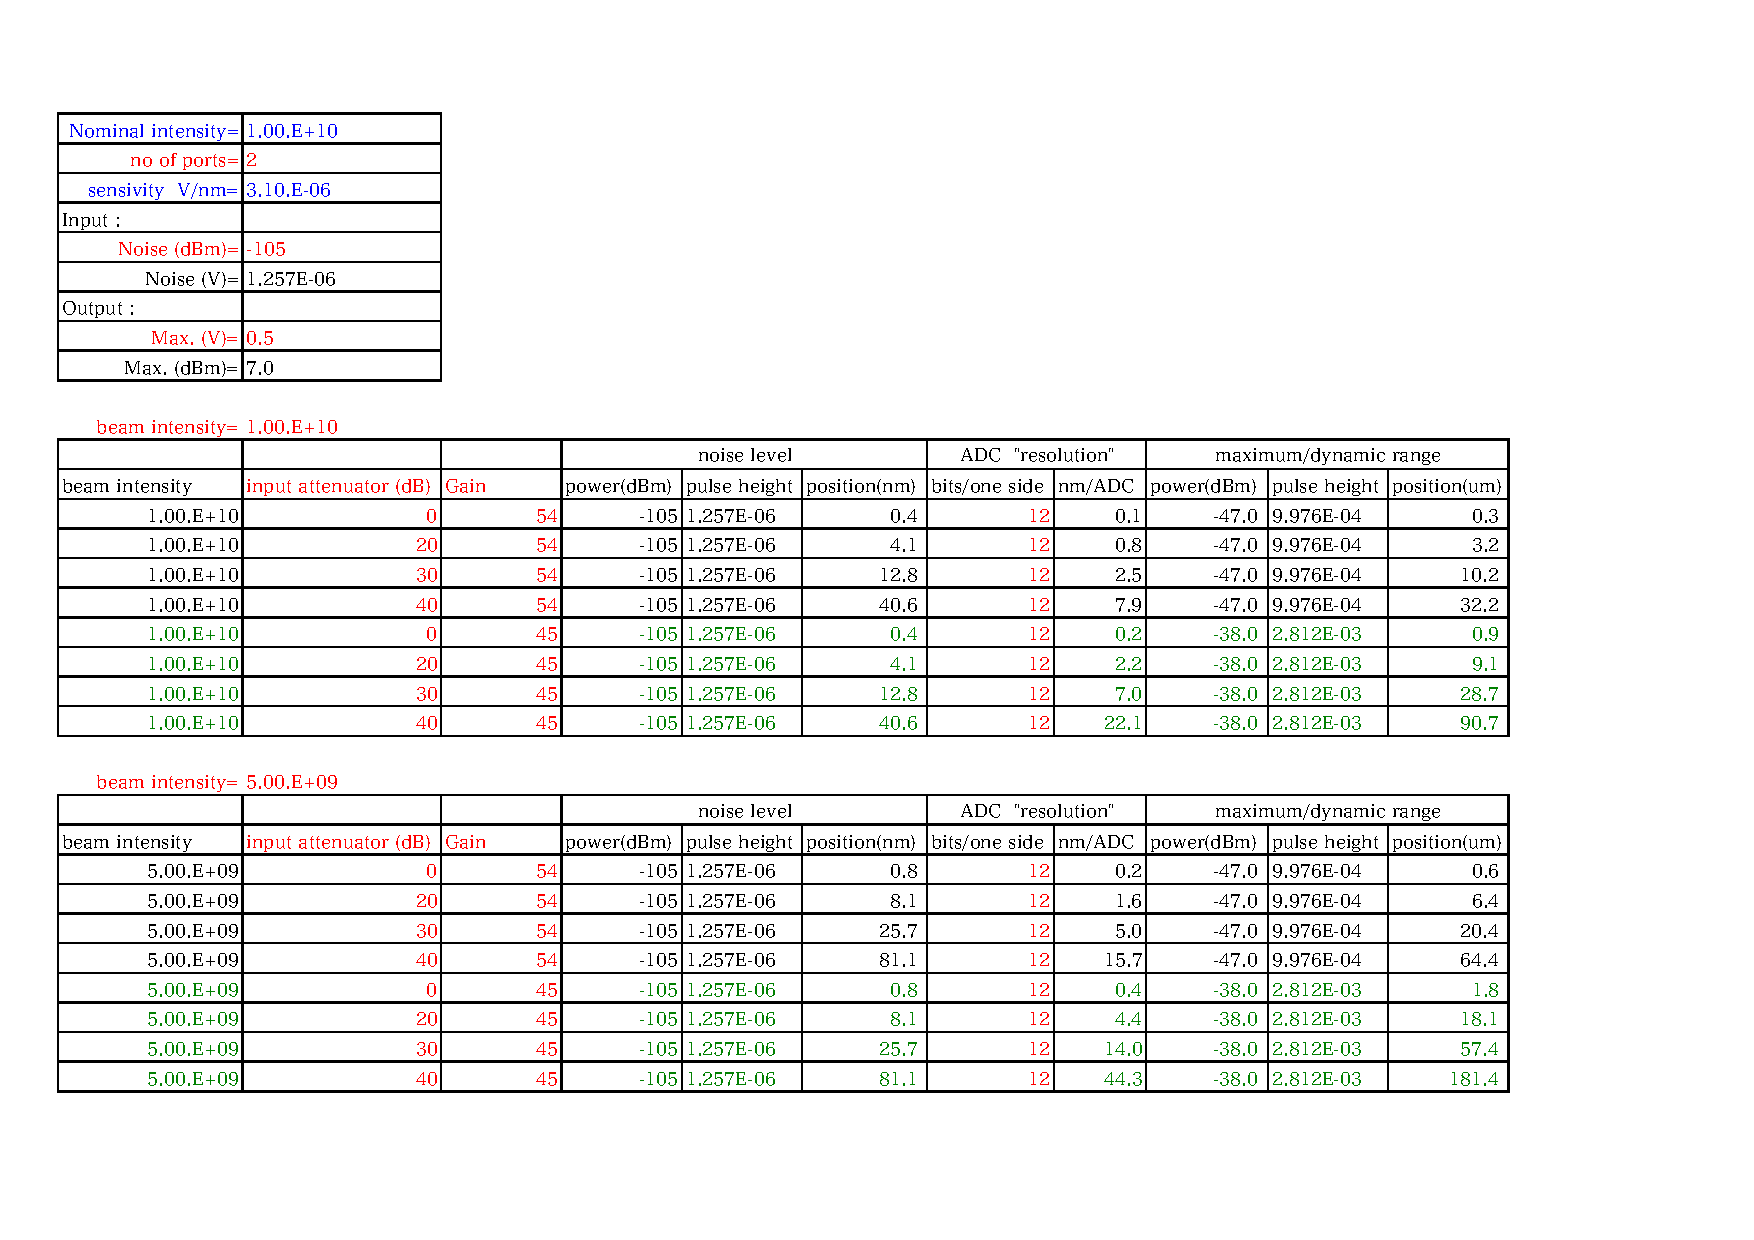
\includegraphics[angle=0,scale=0.7]{dynamic-range-resolution-double-port.pdf}\caption{Dynamic range resolution double port, KNU electronics.}\label{f-dynrange-KNU}
 \end{center}
\end{figure}